\documentclass[unknownkeysallowed]{beamer}
\mode<presentation>
{
%  \usetheme{AnnArbor}
%  \usetheme{Dresden}
%  \usetheme{Montpellier}
%  \usetheme{Antibes}
%  \usetheme{Frankfurt}
%  \usetheme{PaloAlto}
%  \usetheme{Bergen}
%  \usetheme{Boadilla}
%  \usetheme{Goettingen}
%  \usetheme{Pittsburgh}	%!!
%  \usetheme{Berkeley}
%  \usetheme{Hannover}
%  \usetheme{Rochester}		%!!!
%  \usetheme{Berlin}
%  \usetheme{Ilmenau}
%  \usetheme{Singapore}
  \usetheme{Boadilla}		%viel platz
%  \usetheme{JuanLesPins}
%  \usetheme{Szeged}		%!
%  \usetheme{boxes}
%  \usetheme{Luebeck}
%  \usetheme{Warsaw}
%  \usetheme{Copenhagen}
%  \usetheme{Madrid}
%  \usetheme{Darmstadt}
%  \usetheme{Malmoe}
%  \usetheme{default}
%  \usetheme{JuanLesPins}

%  \usetheme{Marburg}


%\usefonttheme{professionalfonts}
%	default | professionalfonts | serif |
%	structurebold | structureitalicserif |
%	structuresmallcapsserif
%\useinnertheme{rounded}
%	circles | default | inmargin |
%	rectangles | rounded

%  \setbeamercovered{transparent}
  % oder auch nicht
\usecolortheme{rose}


\definecolor{uaf yellow}{cmyk}{0,0.16,1,0} % official UAF yellow
\definecolor{light yellow}{cmyk}{0.01,0,0.16,0}
\definecolor{uaf blue}{cmyk}{1,0.66,0,0.02} % official UAF blue
\definecolor{light blue}{cmyk}{0.22,0.11,0,0}
\definecolor{arsc blue}{HTML}{005496}
\definecolor{arsc red}{HTML}{a20a42}
\definecolor{arsc green}{HTML}{009a82}
\definecolor{light gray}{HTML}{777777}

  %navigation aus, klaut nur platz
  \setbeamertemplate{navigation symbols}{}
% Reset title background to default
%\setbeamertemplate{title page}[default]
\setbeamercolor{title}{bg=}
\setbeamercolor{frametitle}{bg=uaf blue, fg=white}
\setbeamercolor{institute}{fg=white}
\setbeamercolor{date}{fg=white}
\setbeamercolor{block}{bg=}
%\setbeamercolor{title}{fg=black}

% Reset block background to default
%\setbeamertemplate{blocks}[default]
%\setbeamercolor{block title}{bg=}
%\setbeamercolor{block body}{bg=}

\beamertemplatenavigationsymbolsempty  
\setbeamertemplate{blocks}[rounded][shadows=false]

\useinnertheme{circles}

}
\usepackage[latin1]{inputenc}
\usepackage{latexsym}
\usepackage{amsfonts}
%\usepackage{natbib}
\usepackage{fancyhdr}
\usepackage{graphicx}
%\usepackage{subfigure}
% oder was auch immer
\usepackage{grffile}
\usepackage{pgf}
\usepackage{tikz}

\usepackage{listings}

\usepackage{times}
\usepackage[T1]{fontenc}
%\usepackage{appendixnumber}
% Oder was auch immer. Zu beachten ist, das Font und Encoding passen
% m�ssen. Falls T1 nicht funktioniert, kann man versuchen, die Zeile
% mit fontenc zu l�schen.

\hypersetup{
    bookmarks=true,         % show bookmarks bar?
    unicode=false,          % non-Latin characters in Acrobat's bookmarks
    pdftoolbar=true,        % show Acrobat's toolbar?
    pdfmenubar=true,        % show Acrobat's menu?
    pdffitwindow=false,     % window fit to page when opened
    pdfstartview={FitH},    % fits the width of the page to the window
    pdftitle={My title},    % title
    pdfauthor={Author},     % author
    pdfsubject={Subject},   % subject of the document
    pdfcreator={Creator},   % creator of the document
    pdfproducer={Producer}, % producer of the document
    pdfkeywords={keyword1} {key2} {key3}, % list of keywords
    pdfnewwindow=true,      % links in new window
    colorlinks=false,       % false: boxed links; true: colored links
    linkcolor=red,          % color of internal links
    citecolor=green,        % color of links to bibliography
    filecolor=magenta,      % color of file links
    urlcolor=cyan           % color of external links
}

\title[PAG]% (optional, nur bei langen Titeln n�tig)
{GEOS 436 / 636\\
Programming and Automation for Geoscientists\\[20pt]
-- Week 06: Data I/O --
}

\author[Grapenthin]% (optional, nur bei vielen Autoren)
{Ronni Grapenthin\\
rgrapenthin@alaska.edu\\
Elvey 413B\\
x7682}
% - Namen m�ssen in derselben Reihenfolge wie im Papier erscheinen.
% - Der \inst{?} Befehl sollte nur verwendet werden, wenn die Autoren
%   unterschiedlichen Instituten angeh�ren.

\institute[UAF] % (optional, aber oft n�tig)
{}
% - Der \inst{?} Befehl sollte nur verwendet werden, wenn die Autoren
%   unterschiedlichen Instituten angeh�ren.
% - Keep it simple, niemand interessiert sich f�r die genau Adresse.

% - Namen m�ssen in derselben Reihenfolge wie im Papier erscheinen.
% - Der \inst{?} Befehl sollte nur verwendet werden, wenn die Autoren
%   unterschiedlichen Instituten angeh�ren.

% - Der \inst{?} Befehl sollte nur verwendet werden, wenn die Autoren
%   unterschiedlichen Instituten angeh�ren.
% - Keep it simple, niemand interessiert sich f�r die genau Adresse.

\date[]{}

% - Volle oder abgek�rzter Name sind m�glich.
% - Dieser Eintrag ist nicht f�r das Publikum gedacht (das wei�
%   n�mlich, bei welcher Konferenz es ist), sondern f�r Leute, die diese
%   Folien sp�ter lesen.

%\AtBeginSection[]
%{
%  \begin{frame}<beamer>
%    \frametitle{Outline}
%    \tableofcontents[currentsection,currentsubsection]
%  \end{frame}
%}

% Falls Aufz�hlungen immer schrittweise gezeigt werden sollen, kann
% folgendes Kommando benutzt werden:

%\beamerdefaultoverlayspecification{<+->}

%%switch on to have only frame numbers
\setbeamertemplate{footline}[frame number]

\defbeamertemplate*{title page}{customized}[1][]
{
		\begin{tikzpicture}
			\node[text width=\textwidth,
				fill=gray!70, 
				fill opacity=0.75,
				text opacity=1,
				rounded corners = 10pt,
				inner sep=2pt]{
				\begin{center}	
			  \usebeamerfont{title}{\bf \usebeamercolor[fg]{title} \inserttitle}
			  \par
			  \usebeamerfont{subtitle}\insertsubtitle\par
			  \bigskip
			  \usebeamerfont{author}\insertauthor\par
			  \bigskip
			  \usebeamerfont{institute}\insertinstitute\par
			  \bigskip
			  \usebeamerfont{date}\insertdate\par
			  \end{center}
			  };
	\end{tikzpicture}		  
%	\vspace{0.4cm}\usebeamercolor[fg]{titlegraphic}\inserttitlegraphic 
%	\begin{flushright}
%	\vspace{-1.25cm}\includegraphics[width=2cm]{../moore_logo_transp.png}\vspace{5cm}
%	\end{flushright}
}

\begin{document}

\lstset{numbers=left, numberstyle=\tiny, stepnumber=2, basicstyle=\ttfamily, numbersep=5pt, xleftmargin=10pt}

\setbeamertemplate{background}{\includegraphics[width=\paperwidth]{/home/roon/Pictures/rooftop_initial.jpg}}

	\begin{frame}
	\begin{center}
		\titlepage
	\end{center}
	\end{frame}

\setbeamertemplate{background}{}

\begin{frame}
\frametitle{}
	\vspace{2cm}
	\begin{center}
		How can you {\bf process your data}\\
		and\\
		{\bf preserve the results} of your work?
	\end{center}
%	\vspace{4cm}
\end{frame}

\begin{frame}
	\frametitle{Data Processing Pipeline}
		\vspace{-0.25cm}
		\begin{center}
			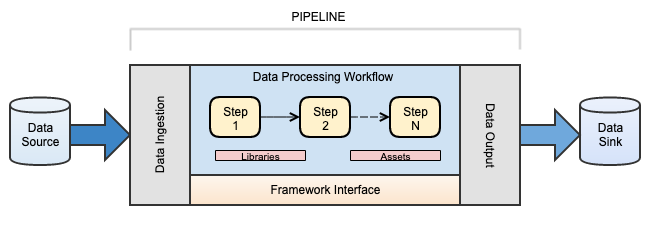
\includegraphics[width=\textwidth]{../figures/pipeline_here_com.png}
		\end{center}
		\begin{flushright}
			\tiny{\emph{\url{here.com}}}
		\end{flushright}
	\begin{center}
		So far, we've dealt with parts of the processing workflow.\\
		Today, we add Data Input (Ingestion) and Output (I/O).
	\end{center}
\end{frame}

\begin{frame}
	\frametitle{Data Storage}
	\begin{itemize}
		\item Storage-needs range from a file with a handful of rows and columns to data distributed over millions of files each with massive amounts of data
		\item {\bf Consistent} formatting of the data allows processing of MANY files with one program
		\item Consistent formatting is difficult for people to do (think hard about format initially!)
		\item Data are stored in a vast range of different data formats
		\item Main categories are: {\bf text-based} (modern Excel {\tt *.xlsx}, other tabulated data {\tt *.csv(x), *.txt, ...}), and {\bf binary} (old Excel {\tt *.xls}, HDF5 {\tt *.h5})
		\item Main difference: text files are human-readable, binary files are not
	\end{itemize}
\end{frame}


\begin{frame}
	\frametitle{Generic Data Ingestion}
	\begin{itemize}
		\item To do anything worthwhile, you {\bf MUST} know your data's format.
		\item Binary?
			\begin{itemize}
				\item Is there a reader for that specific format (e.g., {\tt *.xls})? 
				\item What is the data structure that is being created by that reader?
				\item How do I access data point {\tt x}?
				\item READ THE DOCUMENTATION!
			\end{itemize}
		\item Text-based?
			\begin{itemize}
				\item Is there a reader for that specific format (e.g., {\tt *.xlsx, *.csv})? See above.
				\item Often (NOT always) file contains ``header'' information, one or more lines that explain how the data are formatted, what fields mean etc.
				\item Are all ``columns'' numeric or are there also strings, other types?
				\item Write your own reader for specific formats.
				\item Modern tools (Numpy, Pandas) make that quite easy (one function call)
			\end{itemize}
	\end{itemize}
\end{frame}

\begin{frame}
	\frametitle{Generic Data Output 1/3}
	\begin{itemize}
		\item Data output ranges widely:
			\begin{enumerate}
			\item writing something to the screen 
			\item storing numerical results in a file on disk
			\item make a plot
			\end{enumerate}
		\item Plotting is next week, we focus on (1) and (2)
	\end{itemize}
\end{frame}

\begin{frame}
	\frametitle{Generic Data Output 2/3}
	Output to the screen can be highly effective 
			\begin{itemize}
			\item You can read it (small volumes of output)
			\item You may be able to ``pipe'' the output into another program (more about that in unix tools)
			\item You can redirect it dynamically into a file.
			\end{itemize}
\end{frame}

\begin{frame}
	\frametitle{Generic Data Output 3/3}
	Output to files
			\begin{itemize}
			\item Should happen if the computations take a long time (modeling)
			\item Same things for data formats apply as for reading
			\item Do your best to keep documentation with data (e.g., header lines, self-documenting formats)
			\item It's worth to think about tradeoffs between:
				\begin{itemize}
					\item long-term readability (text files will always be readable)
					\item proprietary data formats (Will you be able to read an Excel file in 30 years?) 
					\item storage efficiency (Is it important that the file is 2MB vs 5MB, 500MB vs 5TB?)
				\end{itemize}
			\end{itemize}
\end{frame}


\begin{frame}
	\frametitle{I/O on the Commandline}
	\begin{columns}[t]
	\column{0.5\textwidth}
		\begin{itemize}	
			\item Listed for completeness. Will be covered at length during the Unix Tools sessions later in the semester.
			\item For now: {\bf There are excellent, time-tested tools available for efficient processing of large quantities of (text-based) data.}

		\end{itemize}
	\column{0.5\textwidth}
		\begin{center}
			
\includegraphics[width=0.7\textwidth]{../figures/data_science_at_the_commandline.png}
		\end{center}
		\begin{flushright}
			\tiny{\emph{O'Reilly\\}}
			\vspace{0.5cm}
		\end{flushright}
	\end{columns}	
	{\scriptsize Read the book for free at {\scriptsize \url{https://www.datascienceatthecommandline.com/1e}}}
\end{frame}

%\begin{frame}
%	\frametitle{I/O on the Commandline: Example}
%	Problem: Observations of some sort in 
%	23 trees with some data in fu
%\end{frame}

\begin{frame}
	\frametitle{I/O in Base Python}
	Output to screen -- {\tt print()}
		\begin{itemize}
		\item We've used this quite a bit, Lab will go over some functionality.
		\item This is an incredibly important tool! Allows your program to give feedback to you.
		\item Put some time into exploring the capabilities.
		\end{itemize}

	\begin{columns}[t]
	\column{0.58\textwidth}
		\begin{block}{}
		{\tiny
		 \lstinputlisting[language=python, numbers=none]{../listings/io_print.py}
		}
		\end{block}
	\column{0.38\textwidth}
		\begin{block}{}
		{\tiny
		 \lstinputlisting[language=bash, numbers=none]{../listings/io_print.txt}
		}
		\end{block}
	\end{columns}
\end{frame}


\begin{frame}
	\frametitle{I/O in Base Python}
	Input:
		\begin{itemize}
		\item Base Python comes with tools to read text, binary files: {\tt open()}
		\item Can read full files or lines {\tt read(), readlines()}
		\item Basic functionality, requires some work to get various files properly read
		\end{itemize}
\end{frame}

\begin{frame}
	\frametitle{I/O in Base Python}
	\vspace{-0.5cm}
	\begin{columns}[t]
	\column{0.48\textwidth}
		\begin{block}{}
		{\tiny
		 \lstinputlisting[language=python, numbers=none]{../listings/io_open.py}
		}
		\end{block}
	\column{0.48\textwidth}
		\begin{block}{}
		{\tiny
		 \lstinputlisting[language=bash, numbers=none]{../listings/io_open.txt}
		}
		\end{block}
	\end{columns}
\end{frame}


\begin{frame}
	\frametitle{I/O in Base Python}
	Output to file:
		\begin{itemize}
		\item Same as input (use {\tt open()} in write {\tt w}, or append {\tt a} mode
		\item Functionality similarly basic, requires some work to get it right
		\end{itemize}

\end{frame}

\begin{frame}
	\frametitle{I/O in Base Python}
	\vspace{-0.5cm}
	\begin{columns}[t]
	\column{0.48\textwidth}
		\begin{block}{}
		{\tiny
		 \lstinputlisting[language=python, numbers=none]{../listings/io_write.py}
		}
		\end{block}
	\column{0.48\textwidth}
		\begin{block}{}
		{\tiny
		 \lstinputlisting[language=bash, numbers=none]{../listings/io_write.txt}
		}
		\end{block}
	\end{columns}
\end{frame}

\begin{frame}
	\frametitle{File Handling with NumPy}
		\begin{center}
			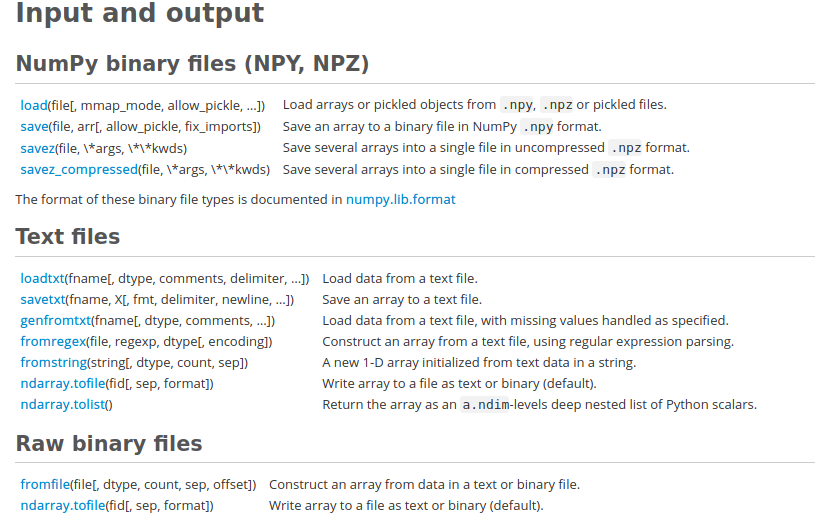
\includegraphics[width=0.9\textwidth]{../figures/numpy_io_routines.png}
		\end{center}
		\begin{flushright}
			\tiny{\emph{numpy.org\\}}
			\vspace{0.5cm}
		\end{flushright}
\end{frame}

\begin{frame}
	\frametitle{File Handling with NumPy}
		\begin{center}
			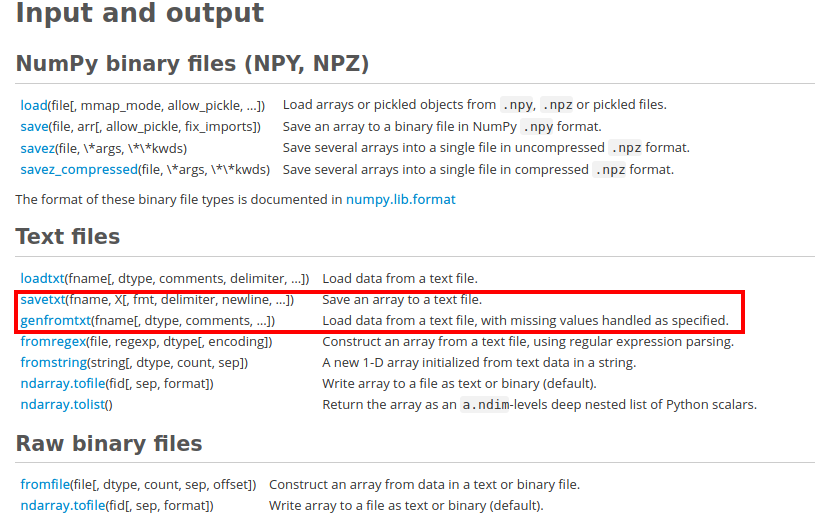
\includegraphics[width=0.9\textwidth]{../figures/numpy_io_routines_marked.png}
		\end{center}
		\begin{flushright}
			\tiny{\emph{numpy.org\\}}
			\vspace{0.5cm}
		\end{flushright}
\end{frame}


\begin{frame}
	\frametitle{Read Textfile with NumPy - genfromtxt }
		\begin{center}
			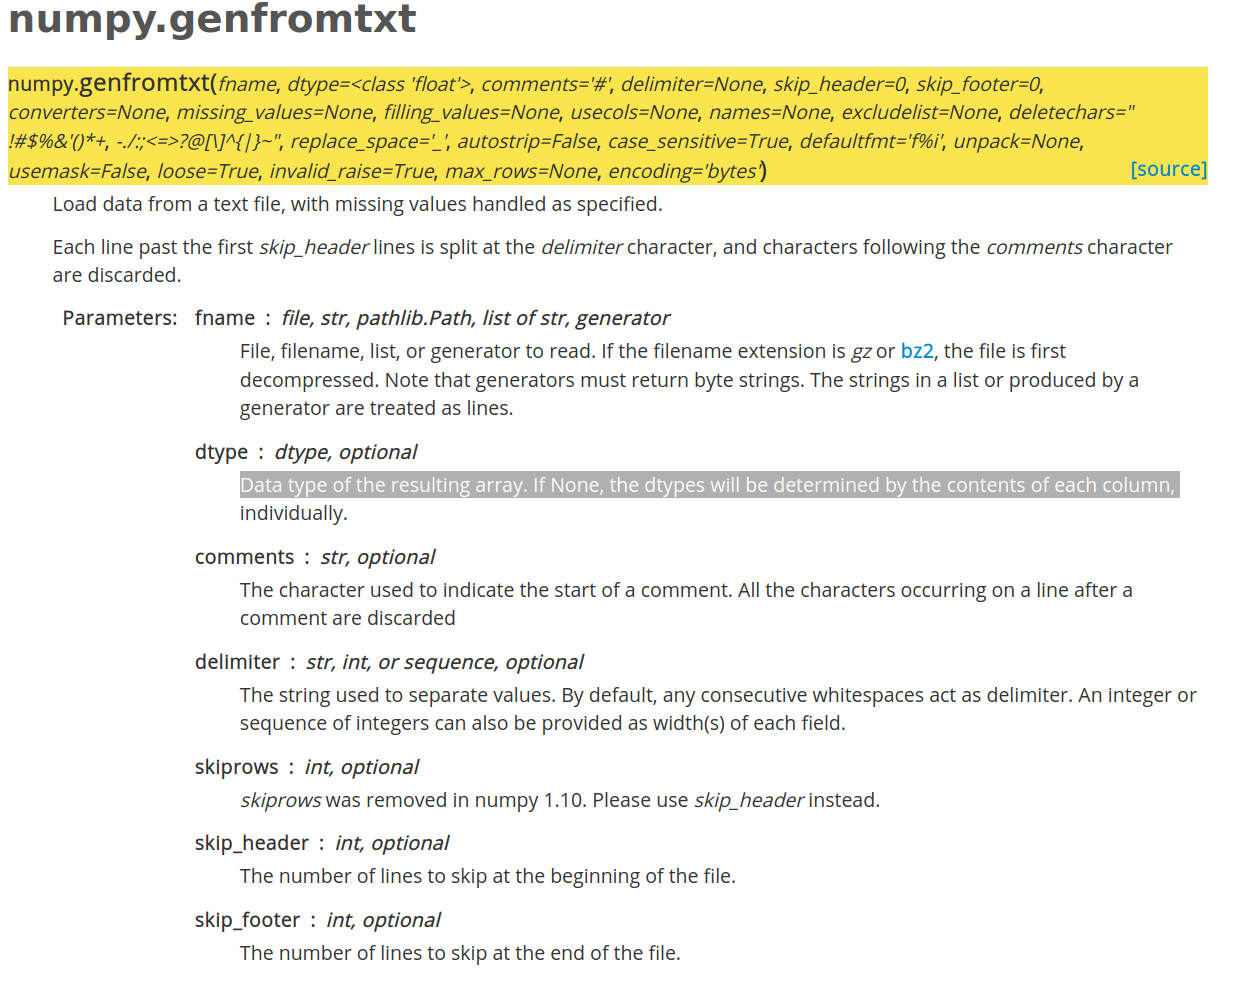
\includegraphics[width=0.8\textwidth]{../figures/numpy_genfromtxt.png}
		\end{center}
		\begin{flushright}
			\vspace{-0.25cm}
			\tiny{\emph{numpy.org\\}}
			\vspace{0.5cm}
		\end{flushright}
\end{frame}

\begin{frame}
	\frametitle{Read Textfile with NumPy - genfromtxt }
	\vspace{-0.5cm}
	\begin{columns}[t]
	\column{0.48\textwidth}
		\begin{block}{}
		{\tiny
		 \lstinputlisting[language=python, numbers=none]{../listings/np_genfromtxt.py}
		}
		\end{block}
	\column{0.48\textwidth}
		\begin{block}{}
		{\tiny
		 \lstinputlisting[language=bash, numbers=none]{../listings/np_genfromtxt.txt}
		}
		\end{block}
	\end{columns}
\end{frame}

\begin{frame}
	\frametitle{Save Textfile with NumPy - savetxt }
		\begin{center}
			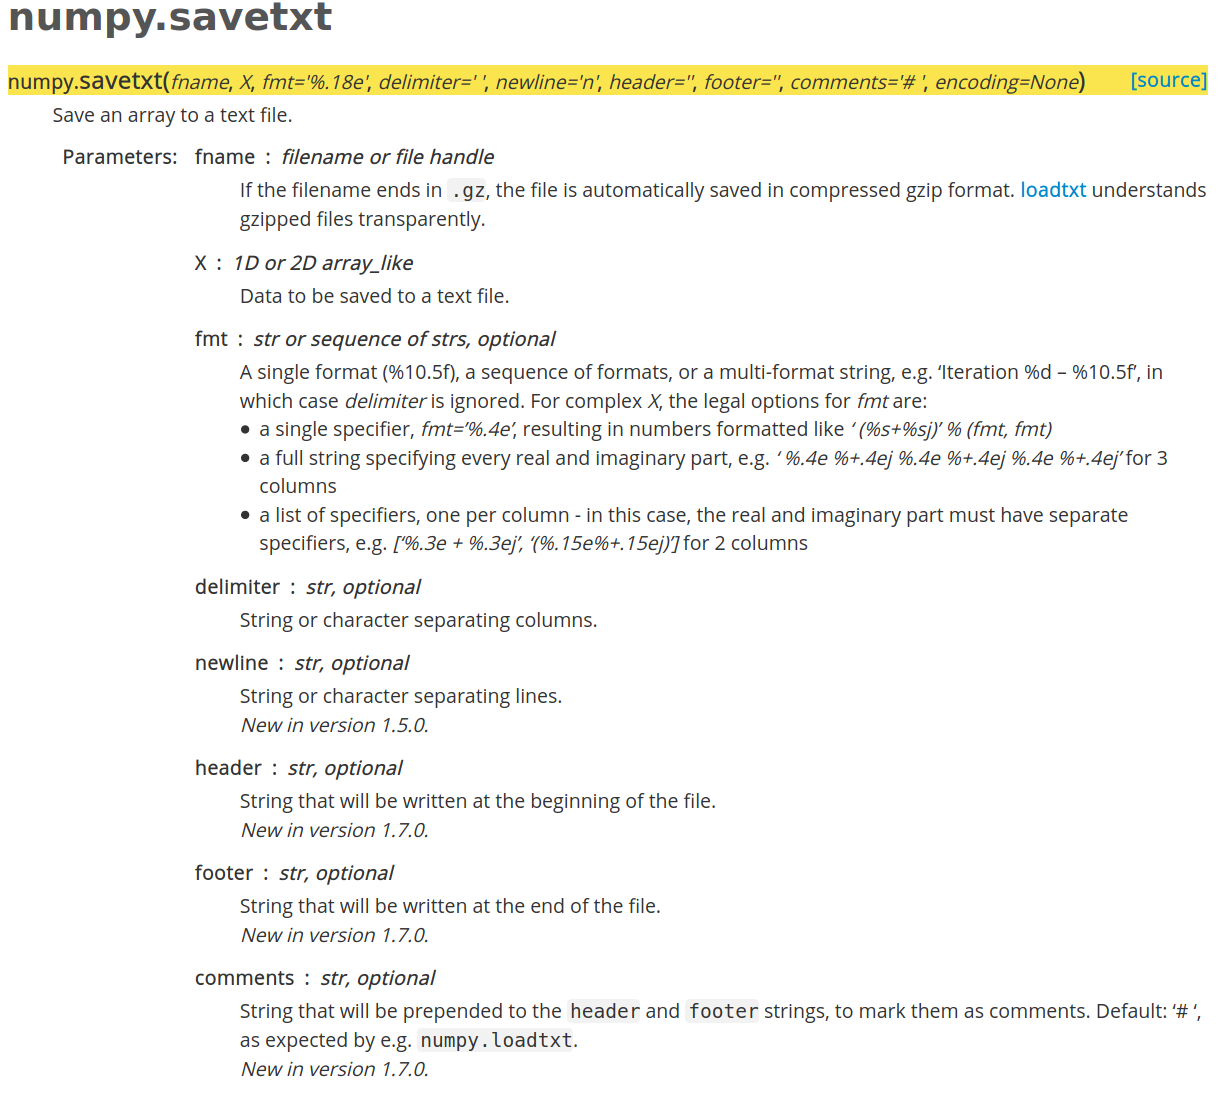
\includegraphics[width=0.75\textwidth]{../figures/numpy_savetxt.png}
		\end{center}
		\begin{flushright}
			\vspace{-0.5cm}
			\tiny{\emph{numpy.org\\}}
			\vspace{0.5cm}
		\end{flushright}
\end{frame}

\begin{frame}
	\frametitle{Read Textfile with NumPy - savetxt }
	\vspace{-0.5cm}
	Eliminate all but three entries from station database, make a new file:
		\begin{block}{}
		{\tiny
		 \lstinputlisting[language=python, numbers=none]{../listings/np_savetxt.py}
		}
		\end{block}
	New file contents:
		\begin{block}{}
		{\tiny
		 \lstinputlisting[language=bash, numbers=none]{../listings/stations_short.txt}
		}
		\end{block}

\end{frame}


\begin{frame}
	\frametitle{File Handling with Pandas}
		\begin{center}
			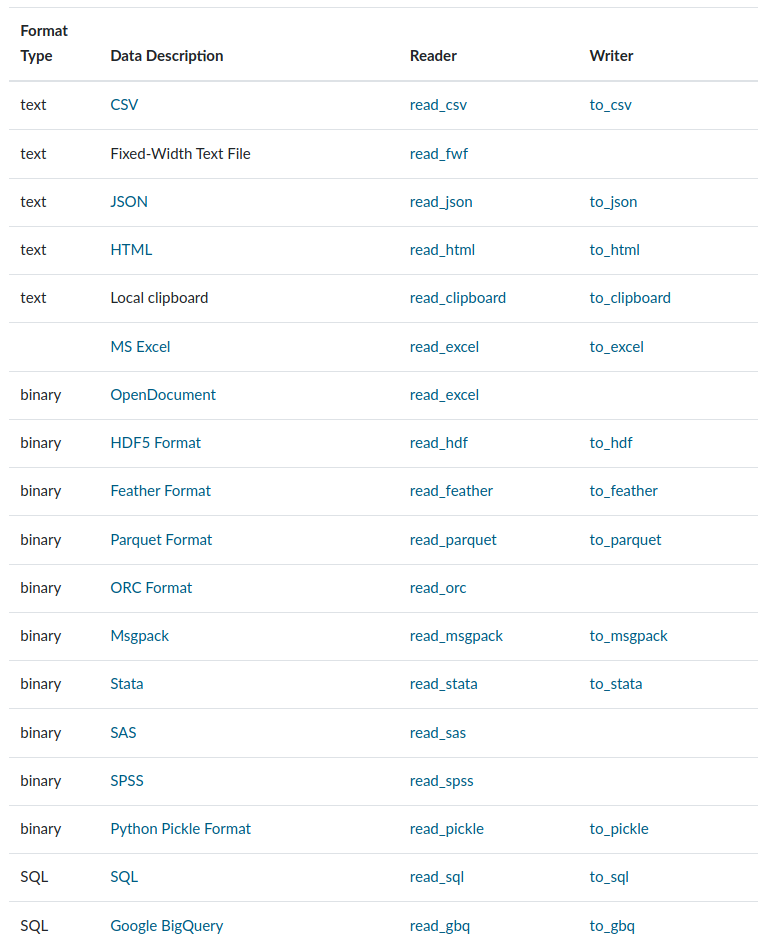
\includegraphics[width=0.55\textwidth]{../figures/pandas_dataio.png}
		\end{center}
		\begin{flushright}
			\vspace{-0.5cm}
			\tiny{\emph{pandas.pydata.org}}
			\vspace{0.5cm}
		\end{flushright}
\end{frame}

\begin{frame}
	\frametitle{File Handling with Pandas}
		\begin{center}
			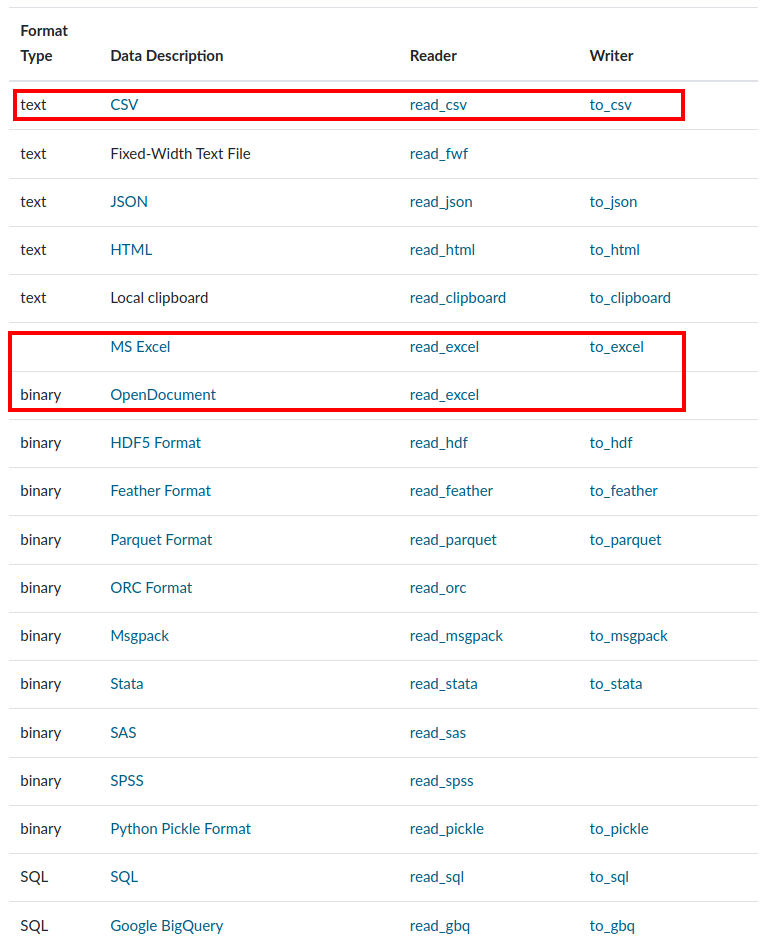
\includegraphics[width=0.55\textwidth]{../figures/pandas_dataio_marked.png}
		\end{center}
		\begin{flushright}
			\vspace{-0.5cm}
			\tiny{\emph{pandas.pydata.org}}
			\vspace{0.5cm}
		\end{flushright}
\end{frame}


\begin{frame}
	\frametitle{Write CSV File with Pandas - read\_csv}
		\begin{block}{}
		{\tiny
		 \lstinputlisting[language=python, numbers=none]{../listings/pandas_read_csv.py}
		}
		\end{block}

		\begin{block}{}
		{\tiny
		 \lstinputlisting[language=bash, numbers=none]{../listings/pandas_read_csv.txt}
		}
		\end{block}

\end{frame}

\begin{frame}
	\frametitle{Write CSV File with Pandas - to\_csv}
	Select three entries from station database, make a new file:
		\begin{block}{}
		{\tiny
		 \lstinputlisting[language=python, numbers=none]{../listings/pandas_to_csv.py}
		}
		\end{block}
	New file contents:
		\begin{block}{}
		{\tiny
		 \lstinputlisting[language=bash, numbers=none]{../listings/stations_short.csv}
		}
		\end{block}

\end{frame}


\end{document}
